\chapter{Chapter XI}

\begin{verse}
1st Outlaw: Stand, sir, and throw us that you have about you;\\
If not, we'll make you sit, and rifle you.\\
Speed: Sir, we are undone! these are the villains\\
That all the travellers do fear so much.\\
Val: My friends,--\\
1st Out: That's not so, sir, we are your enemies.\\
2d Out: Peace! we'll hear him.\\
3d Out: Ay, by my beard, will we;\\
For he's a proper man.\\!
\attrib{--Two Gentlemen of Verona}
\end{verse}

\lettrine{T}{he} nocturnal adventures of Gurth were not yet concluded;
indeed he
himself became partly of that mind, when, after passing one or two
straggling houses which stood in the outskirts of the village, he found
himself in a deep lane, running between two banks overgrown with hazel
and holly, while here and there a dwarf oak flung its arms altogether
across the path. The lane was moreover much rutted and broken up by the
carriages which had recently transported articles of various kinds to
the tournament; and it was dark, for the banks and bushes intercepted
the light of the harvest moon.

From the village were heard the distant sounds of revelry, mixed
occasionally with loud laughter, sometimes broken by screams, and
sometimes by wild strains of distant music. All these sounds, intimating
the disorderly state of the town, crowded with military nobles and their
dissolute attendants, gave Gurth some uneasiness. ``The Jewess was
right,'' he said to himself. ``By heaven and St Dunstan, I would I were
safe at my journey's end with all this treasure! Here are such numbers,
I will not say of arrant thieves, but of errant knights and errant
squires, errant monks and errant minstrels, errant jugglers and errant
jesters, that a man with a single merk would be in danger, much more a
poor swineherd with a whole bagful of zecchins. Would I were out of the
shade of these infernal bushes, that I might at least see any of St
Nicholas's clerks before they spring on my shoulders.''

Gurth accordingly hastened his pace, in order to gain the open common to
which the lane led, but was not so fortunate as to accomplish his
object. Just as he had attained the upper end of the lane, where the
underwood was thickest, four men sprung upon him, even as his fears
anticipated, two from each side of the road, and seized him so fast,
that resistance, if at first practicable, would have been now too
late.--``Surrender your charge,'' said one of them; ``we are the
deliverers of the commonwealth, who ease every man of his burden.''

``You should not ease me of mine so lightly,'' muttered Gurth, whose
surly honesty could not be tamed even by the pressure of immediate
violence,--``had I it but in my power to give three strokes in its
defence.''

``We shall see that presently,'' said the robber; and, speaking to his
companions, he added, ``bring along the knave. I see he would have his
head broken, as well as his purse cut, and so be let blood in two veins
at once.''

Gurth was hurried along agreeably to this mandate, and having been
dragged somewhat roughly over the bank, on the left-hand side of the
lane, found himself in a straggling thicket, which lay betwixt it and
the open common. He was compelled to follow his rough conductors into
the very depth of this cover, where they stopt unexpectedly in an
irregular open space, free in a great measure from trees, and on which,
therefore, the beams of the moon fell without much interruption from
boughs and leaves. Here his captors were joined by two other persons,
apparently belonging to the gang. They had short swords by their sides,
and quarter-staves in their hands, and Gurth could now observe that all
six wore visors, which rendered their occupation a matter of no
question, even had their former proceedings left it in doubt.

``What money hast thou, churl?'' said one of the thieves.

``Thirty zecchins of my own property,'' answered Gurth, doggedly.

``A forfeit--a forfeit,'' shouted the robbers; ``a Saxon hath thirty
zecchins, and returns sober from a village! An undeniable and
unredeemable forfeit of all he hath about him.''

``I hoarded it to purchase my freedom,'' said Gurth.

``Thou art an ass,'' replied one of the thieves ``three quarts of double
ale had rendered thee as free as thy master, ay, and freer too, if he be
a Saxon like thyself.''

``A sad truth,'' replied Gurth; ``but if these same thirty zecchins will
buy my freedom from you, unloose my hands, and I will pay them to you.''

``Hold,'' said one who seemed to exercise some authority over the
others; ``this bag which thou bearest, as I can feel through thy cloak,
contains more coin than thou hast told us of.''

``It is the good knight my master's,'' answered Gurth, ``of which,
assuredly, I would not have spoken a word, had you been satisfied with
working your will upon mine own property.''

``Thou art an honest fellow,'' replied the robber, ``I warrant thee; and
we worship not St Nicholas so devoutly but what thy thirty zecchins may
yet escape, if thou deal uprightly with us. Meantime render up thy trust
for a time.'' So saying, he took from Gurth's breast the large leathern
pouch, in which the purse given him by Rebecca was enclosed, as well as
the rest of the zecchins, and then continued his interrogation.--``Who
is thy master?''

``The Disinherited Knight,'' said Gurth.

``Whose good lance,'' replied the robber, ``won the prize in to-day's
tourney? What is his name and lineage?''

``It is his pleasure,'' answered Gurth, ``that they be concealed; and
from me, assuredly, you will learn nought of them.''

``What is thine own name and lineage?''

``To tell that,'' said Gurth, ``might reveal my master's.''

``Thou art a saucy groom,'' said the robber, ``but of that anon. How
comes thy master by this gold? is it of his inheritance, or by what
means hath it accrued to him?''

``By his good lance,'' answered Gurth.--``These bags contain the ransom
of four good horses, and four good suits of armour.''

``How much is there?'' demanded the robber.

``Two hundred zecchins.''

``Only two hundred zecchins!'' said the bandit; ``your master hath dealt
liberally by the vanquished, and put them to a cheap ransom. Name those
who paid the gold.''

Gurth did so.

``The armour and horse of the Templar Brian de Bois-Guilbert, at what
ransom were they held?--Thou seest thou canst not deceive me.''

``My master,'' replied Gurth, ``will take nought from the Templar save
his life's-blood. They are on terms of mortal defiance, and cannot hold
courteous intercourse together.''

``Indeed!''--repeated the robber, and paused after he had said the word.
``And what wert thou now doing at Ashby with such a charge in thy
custody?''

``I went thither to render to Isaac the Jew of York,'' replied Gurth,
``the price of a suit of armour with which he fitted my master for this
tournament.''

``And how much didst thou pay to Isaac?--Methinks, to judge by weight,
there is still two hundred zecchins in this pouch.''

``I paid to Isaac,'' said the Saxon, ``eighty zecchins, and he restored
me a hundred in lieu thereof.''

``How! what!'' exclaimed all the robbers at once; ``darest thou trifle
with us, that thou tellest such improbable lies?''

``What I tell you,'' said Gurth, ``is as true as the moon is in heaven.
You will find the just sum in a silken purse within the leathern pouch,
and separate from the rest of the gold.''

``Bethink thee, man,'' said the Captain, ``thou speakest of a Jew--of an
Israelite,--as unapt to restore gold, as the dry sand of his deserts to
return the cup of water which the pilgrim spills upon them.''

``There is no more mercy in them,'' said another of the banditti, ``than
in an unbribed sheriffs officer.''

``It is, however, as I say,'' said Gurth.

``Strike a light instantly,'' said the Captain; ``I will examine this
said purse; and if it be as this fellow says, the Jew's bounty is little
less miraculous than the stream which relieved his fathers in the
wilderness.''

A light was procured accordingly, and the robber proceeded to examine
the purse. The others crowded around him, and even two who had hold of
Gurth relaxed their grasp while they stretched their necks to see the
issue of the search. Availing himself of their negligence, by a sudden
exertion of strength and activity, Gurth shook himself free of their
hold, and might have escaped, could he have resolved to leave his
master's property behind him. But such was no part of his intention. He
wrenched a quarter-staff from one of the fellows, struck down the
Captain, who was altogether unaware of his purpose, and had well-nigh
repossessed himself of the pouch and treasure. The thieves, however,
were too nimble for him, and again secured both the bag and the trusty
Gurth.

``Knave!'' said the Captain, getting up, ``thou hast broken my head; and
with other men of our sort thou wouldst fare the worse for thy
insolence. But thou shalt know thy fate instantly. First let us speak of
thy master; the knight's matters must go before the squire's, according
to the due order of chivalry. Stand thou fast in the meantime--if thou
stir again, thou shalt have that will make thee quiet for thy
life--Comrades!'' he then said, addressing his gang, ``this purse is
embroidered with Hebrew characters, and I well believe the yeoman's tale
is true. The errant knight, his master, must needs pass us toll-free. He
is too like ourselves for us to make booty of him, since dogs should not
worry dogs where wolves and foxes are to be found in abundance.''

``Like us?'' answered one of the gang; ``I should like to hear how that
is made good.''

``Why, thou fool,'' answered the Captain, ``is he not poor and
disinherited as we are?--Doth he not win his substance at the sword's
point as we do?--Hath he not beaten Front-de-Boeuf and Malvoisin, even
as we would beat them if we could? Is he not the enemy to life and death
of Brian de Bois-Guilbert, whom we have so much reason to fear? And were
all this otherwise, wouldst thou have us show a worse conscience than an
unbeliever, a Hebrew Jew?''

``Nay, that were a shame,'' muttered the other fellow; ``and yet, when I
served in the band of stout old Gandelyn, we had no such scruples of
conscience. And this insolent peasant,--he too, I warrant me, is to be
dismissed scatheless?''

``Not if THOU canst scathe him,'' replied the Captain.--``Here,
fellow,'' continued he, addressing Gurth, ``canst thou use the staff,
that thou starts to it so readily?''

``I think,'' said Gurth, ``thou shouldst be best able to reply to that
question.''

``Nay, by my troth, thou gavest me a round knock,'' replied the Captain;
``do as much for this fellow, and thou shalt pass scot-free; and if thou
dost not--why, by my faith, as thou art such a sturdy knave, I think I
must pay thy ransom myself.--Take thy staff, Miller,'' he added, ``and
keep thy head; and do you others let the fellow go, and give him a
staff--there is light enough to lay on load by.''

The two champions being alike armed with quarter-staves, stepped forward
into the centre of the open space, in order to have the full benefit of
the moonlight; the thieves in the meantime laughing, and crying to their
comrade, ``Miller! beware thy toll-dish.'' The Miller, on the other
hand, holding his quarter-staff by the middle, and making it flourish
round his head after the fashion which the French call ``faire le
moulinet'', exclaimed boastfully, ``Come on, churl, an thou darest: thou
shalt feel the strength of a miller's thumb!''

\begin{figure}
    \centering
    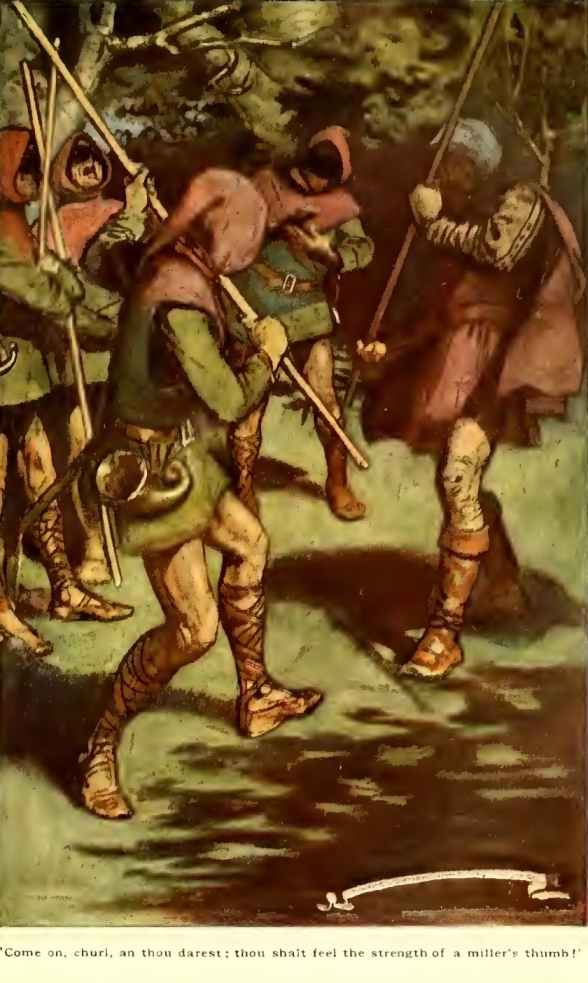
\includegraphics[height=.9\textheight]{ivanhoe/0169m}
    \caption{`Come on, churl, an thou darest; thou shalt feel the
    strength of a miller's thumb!.'}
\end{figure}

``If thou be'st a miller,'' answered Gurth, undauntedly, making his
weapon play around his head with equal dexterity, ``thou art doubly a
thief, and I, as a true man, bid thee defiance.''

So saying, the two champions closed together, and for a few minutes they
displayed great equality in strength, courage, and skill, intercepting
and returning the blows of their adversary with the most rapid
dexterity, while, from the continued clatter of their weapons, a person
at a distance might have supposed that there were at least six persons
engaged on each side. Less obstinate, and even less dangerous combats,
have been described in good heroic verse; but that of Gurth and the
Miller must remain unsung, for want of a sacred poet to do justice to
its eventful progress. Yet, though quarter-staff play be out of date,
what we can in prose we will do for these bold champions.

Long they fought equally, until the Miller began to lose temper at
finding himself so stoutly opposed, and at hearing the laughter of his
companions, who, as usual in such cases, enjoyed his vexation. This was
not a state of mind favourable to the noble game of quarter-staff, in
which, as in ordinary cudgel-playing, the utmost coolness is requisite;
and it gave Gurth, whose temper was steady, though surly, the
opportunity of acquiring a decided advantage, in availing himself of
which he displayed great mastery.

The Miller pressed furiously forward, dealing blows with either end of
his weapon alternately, and striving to come to half-staff distance,
while Gurth defended himself against the attack, keeping his hands about
a yard asunder, and covering himself by shifting his weapon with great
celerity, so as to protect his head and body. Thus did he maintain the
defensive, making his eye, foot, and hand keep true time, until,
observing his antagonist to lose wind, he darted the staff at his face
with his left hand; and, as the Miller endeavoured to parry the thrust,
he slid his right hand down to his left, and with the full swing of the
weapon struck his opponent on the left side of the head, who instantly
measured his length upon the green sward.

``Well and yeomanly done!'' shouted the robbers; ``fair play and Old
England for ever! The Saxon hath saved both his purse and his hide, and
the Miller has met his match.''

``Thou mayst go thy ways, my friend,'' said the Captain, addressing
Gurth, in special confirmation of the general voice, ``and I will cause
two of my comrades to guide thee by the best way to thy master's
pavilion, and to guard thee from night-walkers that might have less
tender consciences than ours; for there is many one of them upon the
amble in such a night as this. Take heed, however,'' he added sternly;
``remember thou hast refused to tell thy name--ask not after ours, nor
endeavour to discover who or what we are; for, if thou makest such an
attempt, thou wilt come by worse fortune than has yet befallen thee.''

Gurth thanked the Captain for his courtesy, and promised to attend to
his recommendation. Two of the outlaws, taking up their quarter-staves,
and desiring Gurth to follow close in the rear, walked roundly forward
along a by-path, which traversed the thicket and the broken ground
adjacent to it. On the very verge of the thicket two men spoke to his
conductors, and receiving an answer in a whisper, withdrew into the
wood, and suffered them to pass unmolested. This circumstance induced
Gurth to believe both that the gang was strong in numbers, and that they
kept regular guards around their place of rendezvous.

When they arrived on the open heath, where Gurth might have had some
trouble in finding his road, the thieves guided him straight forward to
the top of a little eminence, whence he could see, spread beneath him in
the moonlight, the palisades of the lists, the glimmering pavilions
pitched at either end, with the pennons which adorned them fluttering in
the moonbeams, and from which could be heard the hum of the song with
which the sentinels were beguiling their night-watch.

Here the thieves stopt.

``We go with you no farther,'' said they; ``it were not safe that we
should do so.--Remember the warning you have received--keep secret what
has this night befallen you, and you will have no room to repent
it--neglect what is now told you, and the Tower of London shall not
protect you against our revenge.''

``Good night to you, kind sirs,'' said Gurth; ``I shall remember your
orders, and trust that there is no offence in wishing you a safer and an
honester trade.''

Thus they parted, the outlaws returning in the direction from whence
they had come, and Gurth proceeding to the tent of his master, to whom,
notwithstanding the injunction he had received, he communicated the
whole adventures of the evening.

The Disinherited Knight was filled with astonishment, no less at the
generosity of Rebecca, by which, however, he resolved he would not
profit, than that of the robbers, to whose profession such a quality
seemed totally foreign. His course of reflections upon these singular
circumstances was, however, interrupted by the necessity for taking
repose, which the fatigue of the preceding day, and the propriety of
refreshing himself for the morrow's encounter, rendered alike
indispensable.

The knight, therefore, stretched himself for repose upon a rich couch
with which the tent was provided; and the faithful Gurth, extending his
hardy limbs upon a bear-skin which formed a sort of carpet to the
pavilion, laid himself across the opening of the tent, so that no one
could enter without awakening him.
